% Copyright (C) Huawei Technologies Co., Ltd. 2024. All rights reserved.
% SPDX-License-Identifier: MIT
\PassOptionsToClass{handout}{beamer}
\documentclass[aspectratio=169]{beamer}

\usetheme{huawei}
\usepackage{lmodern}
\usepackage{adjustbox}
\usepackage{booktabs}
\usepackage{listings}
\usepackage{pifont}
\usepackage{soul}
\usepackage{tikz}
\usepackage{underscore}
\usepackage{varwidth}
\usepackage{xspace}

%%%%%%%%%%%%%%%%%%%%%%%%%%%%%%%%%%%%%%%%%%%%%%%%%%%%%%%%%%%%%%%%%%%%%%%%%%%%%%%%%
%% colors
%%%%%%%%%%%%%%%%%%%%%%%%%%%%%%%%%%%%%%%%%%%%%%%%%%%%%%%%%%%%%%%%%%%%%%%%%%%%%%%%%
\colorlet{blackish}{black!60}
\colorlet{blueish}{blue!60!black!20}
\colorlet{blueText}{blue!60!black!50}
\colorlet{grayish}{black!10}
\colorlet{greenish}{green!70!black!50}
\colorlet{light gray}{gray!10}
\colorlet{magentish}{magenta!50!black!50}
\colorlet{olivish}{olive!50!black!50}
\colorlet{orangeish}{orange!60!black!30}
\colorlet{redish}{red!60!black!60}

\definecolor{HuaweiRed}{RGB}{237,28,36}
\definecolor{darkred}{RGB}{184, 5, 69}
\definecolor{pltblue}{HTML}{0173B2}
\definecolor{pltgreen}{HTML}{029E73}
\definecolor{pltred}{HTML}{D55E00}
\definecolor{pltpurple}{HTML}{CC78BC}
\colorlet{libvsync}{pltpurple}
\colorlet{vsyncer}{pltblue}

\newcommand{\hide}{\color{gray!70}}
\newcommand{\unhide}{\color{black}}

%%%%%%%%%%%%%%%%%%%%%%%%%%%%%%%%%%%%%%%%%%%%%%%%%%%%%%%%%%%%%%%%%%%%%%%%%%%%%%%%%
%% listings
%%%%%%%%%%%%%%%%%%%%%%%%%%%%%%%%%%%%%%%%%%%%%%%%%%%%%%%%%%%%%%%%%%%%%%%%%%%%%%%%%
\lstdefinestyle{compact}{
	basicstyle=\scriptsize\ttfamily\color{black},
	keywordstyle=\scriptsize\color{blue}\ttfamily,
	commentstyle=\scriptsize\color{gray}\ttfamily,
	stringstyle=\scriptsize\color{darkred}\ttfamily,
	numberstyle=\tiny\color{gray},
	columns=fullflexible,
	tabsize=2,
	showstringspaces=false,
	moredelim=**[is][\color{darkred}]{@}{@},
}

\lstset{
	language=C,
	basicstyle=\scriptsize\ttfamily,
	keywordstyle=\scriptsize\color{darkred}\ttfamily,
	commentstyle=\scriptsize\color{gray!60}\ttfamily,
	moredelim=**[is][\color{pltblue}\tiny]{|}{|},
	escapechar=@,
}
%%%%%%%%%%%%%%%%%%%%%%%%%%%%%%%%%%%%%%%%%%%%%%%%%%%%%%%%%%%%%%%%%%%%%%%%%%%%%%%%%
%% tikz
%%%%%%%%%%%%%%%%%%%%%%%%%%%%%%%%%%%%%%%%%%%%%%%%%%%%%%%%%%%%%%%%%%%%%%%%%%%%%%%%%

\usetikzlibrary{
	decorations.markings,
	decorations.pathmorphing,
	decorations.pathreplacing,
	fit, spy, shapes, intersections, arrows,
	positioning, calc,
	shapes.geometric,
}
\tikzset{
	alt/.code args={<#1>#2#3}{%
		\alt<#1>{\pgfkeysalso{#2}}{\pgfkeysalso{#3}}
	},
	fill on/.style 2 args={alt=#1{fill=#2}{}},
	warning/.style={fill=redish, text=white, font=\bf, rounded corners},
	between/.style args={#1 and #2}{
		at = ($(#1)!0.5!(#2)$)
	},
	alice/.style={draw=olive, very thick},
	alicetxt/.style={alice, text=olive, font=\Large, rounded corners},
	bob/.style={draw=magenta, very thick},
	bobtxt/.style={bob, text=magenta, font=\Large, rounded corners},
}
\newcommand{\coord}[1]{%
	\tikz[remember picture]\coordinate[yshift=1mm,xshift=-2mm] (#1);
}

%%%%%%%%%%%%%%%%%%%%%%%%%%%%%%%%%%%%%%%%%%%%%%%%%%%%%%%%%%%%%%%%%%%%%%%%%%%%%%%%%
%% Text commands
%%%%%%%%%%%%%%%%%%%%%%%%%%%%%%%%%%%%%%%%%%%%%%%%%%%%%%%%%%%%%%%%%%%%%%%%%%%%%%%%
\newcommand{\eg}{eg}
\newcommand{\xmark}{\text{\ding{55}}}

\newcommand{\libvsync}{{\color{libvsync}\texttt{libvsync}}\xspace}
\newcommand{\vsyncer}{{\color{vsyncer}{\texttt{vsyncer}}}\xspace}
\newcommand{\award}[1][1mm]{\hspace{2mm}\tikz[overlay]\node[yshift=#1]{
\includegraphics[width=1.4mm]{figs/award}};\hspace{2mm}}
\newcommand{\bestpaper}{\award{\em\tiny Best Paper}}
\newcommand\battery[1]{\tikz[overlay]\node{
\includegraphics[width=#1]{figs/battery.png}};\,\xspace}
\newcommand\robot[1]{\tikz[overlay]\node{
\includegraphics[width=#1]{figs/smart-robot.jpg}};\,\xspace}
\newcommand\theframerange{0-}
\newcommand\framerange[1]{\renewcommand\theframerange{#1}}
\newcommand{\arm}{ARMv8}
\newcommand{\riscv}{RISC-V}

%%%%%%%%%%%%%%%%%%%%%%%%%%%%%%%%%%%%%%%%%%%%%%%%%%%%%%%%%%%%%%%%%%%%%%%%%%%%%%%%%
%% beamer
%%%%%%%%%%%%%%%%%%%%%%%%%%%%%%%%%%%%%%%%%%%%%%%%%%%%%%%%%%%%%%%%%%%%%%%%%%%%%%%%%
\setbeamertemplate{navigation symbols}{}
\newcommand\nofootline{\setbeamertemplate{footline}{}}
\newcommand\setfootline{\setbeamertemplate{footline}
{%
	\tikz[overlay]%
	\node[font=\tiny, text=black!40, text width=\textwidth-5mm, anchor=west]
	at (2mm, 2mm)
	{%
		\url{vsync@huawei.com} \hspace{15mm}
		Safe and Scalable System Software Concurrency (S4C) Team
		\hfill\insertframenumber/\inserttotalframenumber%
	};
}}

%%%%%%%%%%%%%%%%%%%%%%%%%%%%%%%%%%%%%%%%%%%%%%%%%%%%%%%%%%%%%%%%%%%%%%%%%%%%%%%%%
%% front page
%%%%%%%%%%%%%%%%%%%%%%%%%%%%%%%%%%%%%%%%%%%%%%%%%%%%%%%%%%%%%%%%%%%%%%%%%%%%%%%%%
\title{\huge VSync: Verification and Optimization of\\[2pt]
	Concurrent Algorithms on WMMs\\[4pt]~}
\author{{\small Diogo Behrens --- Huawei Dresden Research Center}}
\institute{}
\date{{\color{black!50}\scriptsize Vsyncer Tutorial @ OSS'24}}

%%%%%%%%%%%%%%%%%%%%%%%%%%%%%%%%%%%%%%%%%%%%%%%%%%%%%%%%%%%%%%%%%%%%%%%%%%%%%%%%
%% Document
%%%%%%%%%%%%%%%%%%%%%%%%%%%%%%%%%%%%%%%%%%%%%%%%%%%%%%%%%%%%%%%%%%%%%%%%%%%%%%%%
\begin{document}

\maketitle
\setfootline
\framerange{1-}

\section{Introduction}
% Copyright (C) Huawei Technologies Co., Ltd. 2024. All rights reserved.
% SPDX-License-Identifier: MIT
\begin{frame}<\theframerange>{As the hardware evolves, so does the concurrency control}
    \begin{columns}
        \column{.6\textwidth}{%
            \begin{block}{Challenges of modern hardware}
                \begin{itemize}\small
                    \item Many-cores everywhere
                    \item<2-> Weak Memory Models, \eg, RISC-V, ARMv8
                    \item<5-> Deep NUMA hierarchies
                    \item<6-> Heterogeneous cores, \eg, big.LITTLE
                \end{itemize}
            \end{block}
        \uncover<7->{%
        \begin{block}{Consequences to concurrent software}
            \begin{itemize}\small
                \item<1-> {Smarter} concurrency is more complex
                \item<8-> {Complexity gets out of control!}
                \item<8-> {\bf Safety compromised:}\\
                    crashes, data corruption, \ldots
            \end{itemize}
        \end{block}}
        }\column{.4\textwidth}{%
            \centering
            \resizebox{\textwidth}{!}{%
            \tikz[align=center,
                n/.style = {ultra thick, line width = 1mm, font=\Large, draw=black, rounded corners, fill=grayish, minimum width=3cm},
                a/.style = {->, line width=2mm},
                news/.style = {draw, very thick, inner sep = 0},
            ]{%
                \draw[use as bounding box, draw=none, dotted] (-5mm, -100mm) rectangle (120mm, 10mm);

                \node<1->[n, fill=blueish] at (-10mm, 10mm)   (hw)  {Multicore\\CPUs};
                \node<1> [right=5mm of hw, yshift=-15mm] (num) {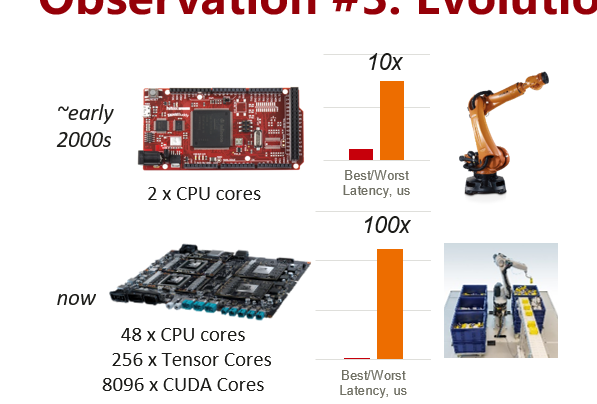
\includegraphics[width=120mm, clip, trim=0 0 0 20]{figs/hardware-evolution.png}};
                \node<2->[right=10mm of hw, yshift=2mm] (num) {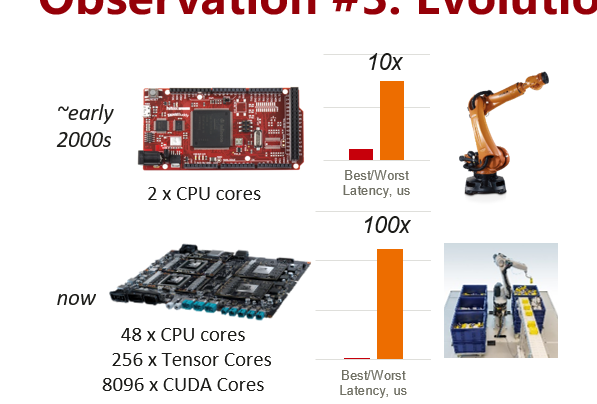
\includegraphics[width=60mm, clip, trim=0 0 0 20]{figs/hardware-evolution.png}};

                \node<2->[n, fill=orangeish, below=35mm of hw] (sw)  {Weak\\Memory};
                \draw<2->[a] (hw) -- (sw);

                \node<3- >[right=10mm of sw] (mp) {\scalebox{1.2}{% Copyright (C) Huawei Technologies Co., Ltd. 2024. All rights reserved.
% SPDX-License-Identifier: MIT
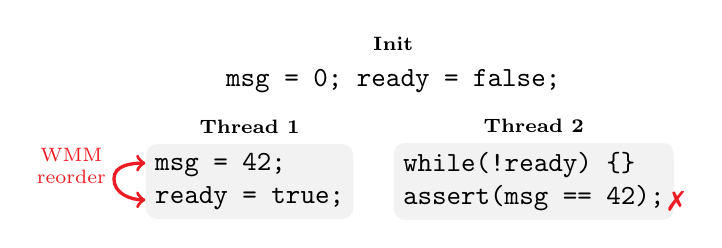
\begin{tikzpicture}[
    a/.style = {->, thick},
    j/.style = {fill=white, font=\scriptsize\bf},
    b/.style = {rounded corners, align=left}, %, text width = 7mm},
    i/.style = {b},
    t/.style = {b, fill=light gray},
    c/.style = {b, fill=light red, text width=34mm},
    ]
\coordinate (x);
\node[i, above=10mm of x] (a) {\verb|msg = 0; ready = false;|};
\node[t, left=5mm of x] (b1) {\verb|msg = 42;|\\ \verb|ready = true;|};
\node[t, right=0mm of x] (b2) {\verb|while(!ready) {}|\\{\verb|assert(msg == 42);|}};
%\node[c, below=of x] (c) {\verb+assert(a != 0 || b != 0);+};
%\draw[a]  (a) -- (b1);
%\draw[a]  (a) -- (b2);
%\draw[a]  (b1) -- (c);
%\draw[a]  (b2) -- (c);
%\node[j, below=1mm of a] {{\tt pthread_create}};
%\node[j, above=1mm of c] {{\tt pthread_join}};
\node[j, above=0 of a] {Init};
\node[j, fill=none, above=0 of b1] (t1) {Thread 1};
\node[j, fill=none, above=0 of b2] (t2) {Thread 2};
\node[text=HuaweiRed, right=-2mm of b2.south east, yshift=2.5mm] {\xmark};

%\draw[a]  (a) -- (t1);
%\draw[a]  (a) -- (t2);
\draw<1->[<->, very thick, HuaweiRed] (b1.170) to [out=180, in = 90]
node[midway, left=1mm, align=center, font=\scriptsize] {WMM\\reorder}
+(-4mm, -2mm) to [out = -90, in = 180] (b1.190);
\end{tikzpicture}
}};

                \node<4->[n, fill=greenish, below=35mm of sw] (alg)  {Heterogeneous\\Cores/Memory};
                \draw<4->[a] (sw) -- (alg);

                \node<5->[right=20mm of alg] (num) {\resizebox{90mm}{!}{% Copyright (C) Huawei Technologies Co., Ltd. 2024. All rights reserved.
% SPDX-License-Identifier: MIT
\begin{tikzpicture}[myarrow/.style={double arrow, draw=none},
  sysbase/.style = {rounded corners, font=\bf, align=left, anchor=center},
    system/.style = {sysbase, draw, dashed},
    proc/.style = {sysbase, fill=grayish, solid, very thick, minimum width=4cm},
    numa/.style = {sysbase, fill=blueish, minimum width=1cm},
    core/.style = {sysbase, fill=white, minimum width=20mm, align=left},
    ]

  \node[system] (nsys) {%
    \begin{tikzpicture}
      \node[proc] (p1) {
        Processor 1\\[4pt]
        \begin{tikzpicture}
          \node[numa] (n1) {Numa 1\\[4pt]
            \begin{tikzpicture}
              \node[core] (c1) {Core 1};
              \node[core, below=1mm of c1] (c2) {Core 2};
              \node[core, below=1mm of c2] (c3) {Core 3};
              \node[core, below=1mm of c3] (c4) {Core 4};
            \end{tikzpicture}
          };
          \node[numa, right=2mm of n1]{Numa 2\\[4pt]
              \begin{tikzpicture}
                \node[core] (c1) {Core 5};
                \node[core, below=1mm of c1] (c2) {Core 6};
                \node[core, below=1mm of c2] (c3) {Core 7};
                \node[core, below=1mm of c3] (c4) {Core 8};
              \end{tikzpicture}
          };
        \end{tikzpicture}
      };
      \node[proc, right=2mm of p1] (p2) {
        Processor 2\\[4pt]
        \begin{tikzpicture}
          \node[numa] (n1) {Numa 2\\[4pt]
            \begin{tikzpicture}
              \node[core] (c1) {Core 9~};
              \node[core, below=1mm of c1] (c2) {Core 10};
              \node[core, below=1mm of c2] (c3) {Core 11};
              \node[core, below=1mm of c3] (c4) {Core 12};
            \end{tikzpicture}
          };
          \node[numa, right=2mm of n1]{Numa 3\\[4pt]
              \begin{tikzpicture}
                \node[core] (c1) {Core 13};
                \node[core, below=1mm of c1] (c2) {Core 14};
                \node[core, below=1mm of c2] (c3) {Core 15};
                \node[core, below=1mm of c3] (c4) {Core 16};
              \end{tikzpicture}
          };
        \end{tikzpicture}
        };
    \end{tikzpicture}
  };
  \node[above=3mm of nsys.north, anchor=center]{Many-core NUMA System};

  \draw<1->[<->, ultra thick, rounded corners, pltgreen,line width=4pt ]
  ($(nsys.north west) + (5mm,-16mm)$)
  to [bend right]
  node[midway, below left=-2mm and 4mm, font=\bf\huge, text=pltgreen, rounded corners] {fast}
  +(-8mm,-3.5mm)
  to [bend right]
  ($(nsys.north west) + (5mm,-23mm)$)
  ;

  \draw<1->[<->, ultra thick, rounded corners, pltred,line width=4pt ]
  ($(nsys.north west) + (38mm,-38mm)$)
  to [out=-90, in=-90]
  node[midway, below=0mm, font=\bf\huge, text=pltred, rounded corners] {slow}
  %+(15mm,-10mm)
  %to [out=0, in=-90]
  ($(nsys.north west) + (68mm,-38mm)$)
  ;

\end{tikzpicture}

}};
                \node<6->[above=-22mm of num.south west, xshift=5mm] {
\includegraphics[width=6cm]{figs/fast-car.png}};
                \node<6->[above=1mm of num.south east] {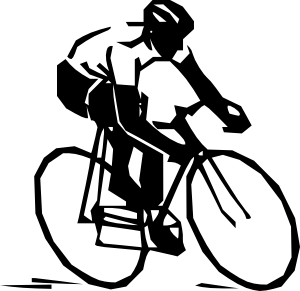
\includegraphics[width=2cm]{figs/bike.png}};

                \node<8->[below left=0mm and 2mm of alg] (boom){
\includegraphics[width=50mm]{figs/explosion.png}};
                \draw<8->[a, decorate, decoration={snake, post length=4mm, segment length = 5mm, amplitude = .5mm }] (alg) to[out=-90, in=0] (boom);

            }
            }
        }
    \end{columns}
\end{frame}

% Copyright (C) Huawei Technologies Co., Ltd. 2024. All rights reserved.
% SPDX-License-Identifier: MIT

\begin{frame}{What can the industry do?}
    \begin{columns}[t]
        \column{.5\textwidth}{\uncover<1->{%
        \begin{center}
            %\hspace{-3mm}
            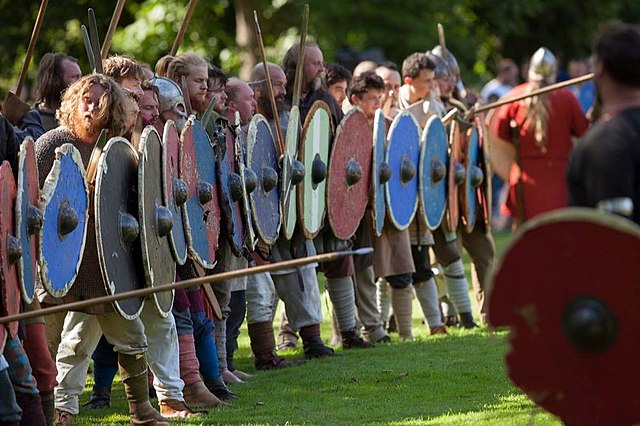
\includegraphics[trim=0 0 32mm 0, clip, width=40mm]{figs/shieldwall}
            \vspace{-4mm}
        \end{center}
        \begin{block}{Keep-it-simple and Overprotect?}
            \begin{itemize}\small\setlength\itemindent{-1em}\setlength\itemsep{1mm}
                \item Simplify design as much as possible
                \item Spray code with memory barriers and locks
                %The musl and MySQL projects conservatively overprotect the code by adding many strong barriers.
                %Depending on the hardware, the additional barriers may hurt performance.
                \item Risk: {\bf performance impact}
            \end{itemize}
        \end{block}}
        } \column{.5\textwidth} {\uncover<1->{%
        \begin{center}
            %\hspace{-3mm}
            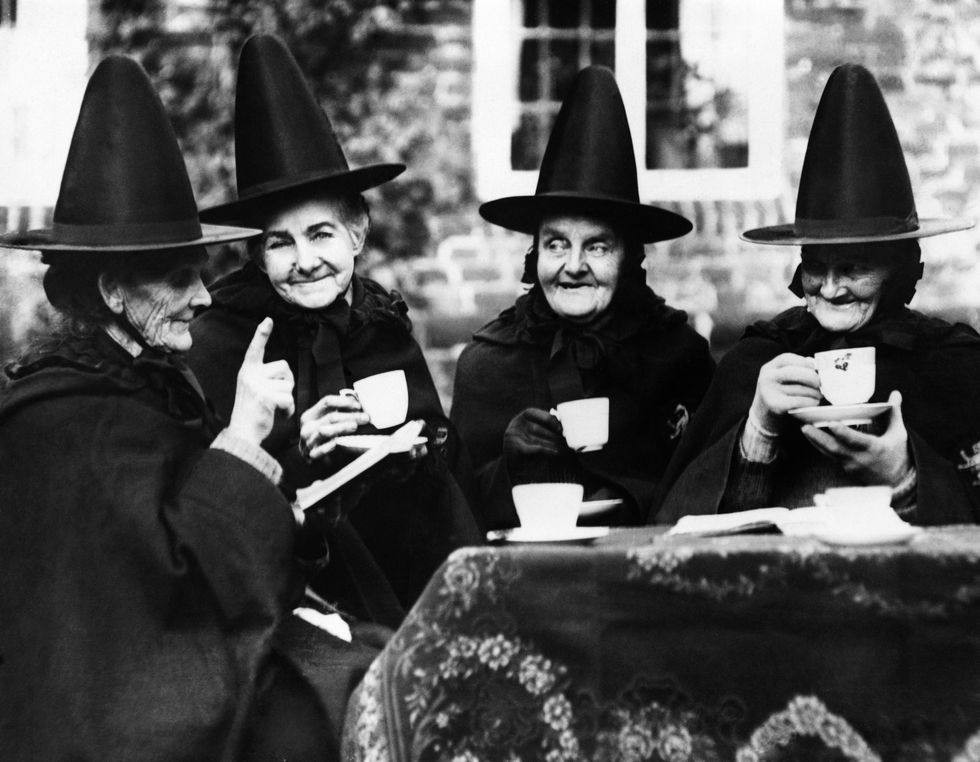
\includegraphics[trim=0 0 0 0, clip, width=40mm]{figs/witches}
            \vspace{-4mm}
        \end{center}
        \begin{block}{Rely on Expert Optimizations?}
            \begin{itemize}\small\setlength\itemindent{-1em}\setlength\itemsep{1mm}
                \item Exclusively rely on highly-skilled engineers
                \item Carefully design, implement and optimize
                \item Risk: {\bf error-prone, low maintainability}
            \end{itemize}
            %Over the course of 6 years, the Linux qspinlock was optimized by
            %highly-skilled engineers.
            %Still, one bug kept dormant during 12 releases.
        \end{block}}
        }
    \end{columns}
\end{frame}

% Copyright (C) Huawei Technologies Co., Ltd. 2024. All rights reserved.
% SPDX-License-Identifier: MIT
\begin{frame}<\theframerange>[fragile]{The VSync Project}
\setul{3pt}{.6pt}

\begin{tikzpicture}[n/.style={text width = .42\textwidth}]
	\node (a) {};

        \node[left=0mm of a] (b) {
\includegraphics[width=6mm]{figs/battery.png}};
        \node[n, above right=5mm and -2mm of a, anchor=north west] (t1) {%
	        \begin{block}{\color{libvsync}\Large Batteries Included}
		\url{github.com/open-s4c/libvsync}

		~\\
		\uncover<2->{%
			{\color{redish}\bf Don't rely on} a minimal set of
			{\color{redish}\bf overprotected and inefficient}
			concurrent components.\\[10pt]}
		\uncover<3->{%
			Instead, {\color{libvsync}\bf provide an efficient
			and verified library} of practical components.
			\only<4->{\bf (WIP)}}
		\end{block}
	};

	\node[right=55mm of a] (c) {
\includegraphics[width=18mm]{figs/smart-robot.jpg}};
	\node[n, above right=5mm and 72mm of a, anchor=north west] {%
		\begin{block}{\color{vsyncer}\Large Automated Experts}
		\url{github.com/open-s4c/vsyncer}

		~\\
		\uncover<5->{%
			{\color{redish}\bf Avoid always relying on}
			concurrency {\color{redish}\bf experts}!\\[10pt]}
		\uncover<6->{%
			Instead, {\color{vsyncer}\bf enable normal
			programmers} to develop concurrent code supported
			by {\color{vsyncer}\bf verification tools}.}
		\end{block}
	};
\end{tikzpicture}

\end{frame}


\section{Concurrency}
\begin{frame}{}
	\begin{columns}[T]
	\column{.49\textwidth}{%
		\begin{block}{{\Large Agenda}}%
		\begin{itemize}\Large
			\item {\hide Introduction}
			\item {\unhide Part 1: Concurrent Monalisa}
			\item {\hide Part 2: {\tt vsyncer} to the rescue}
			\item {\hide Outlook}
		\end{itemize}
		\end{block}
	}\hfill\column{.49\textwidth}{%
		{\setbeamertemplate{blocks}[rounded][shadow=true]%
		 \setbeamercolor{block title}{bg=HuaweiRed, fg=white}%
		 \setbeamercolor{block body}{bg=redish!5}%
		\begin{block}<2->{\Large Coding on your own}%
			\url{github.com/open-s4c/vsyncer-demo}

			~\\

			\begin{itemize}\small
			\item Works best: Linux + Docker
			\item Part 2 only: Windows + Docker
			\item Works: macOS + Docker
			\end{itemize}

			~\\
		\end{block}}
	}
	\end{columns}
\end{frame}

% Copyright (C) Huawei Technologies Co., Ltd. 2024. All rights reserved.
% SPDX-License-Identifier: MIT
\begin{frame}[fragile]{Let's implement a concurrent {\tt cat}}

	\begin{center}
	\begin{tikzpicture}[%
		itemsz/.style={minimum width = 5mm, minimum height = 5mm},
		item/.style={very thick, draw=blackish, itemsz, outer sep=0},
		cursor/.style={very thick,<-, font=\ttfamily},
		TP/.style={rounded corners, ultra thick, draw=olivish, text=olivish},
		TC/.style={rounded corners, ultra thick, draw=magentish, text=magentish},
	]%

	\node[font=\Large\tt] at (0, 45mm) {\$ ccat monalisa.jpg | viu -};

	\node[item, fill on={<1->}{magentish}] at (0, 10mm) (a1) {};
	\node[item, fill on={<1->}{olivish}, right=0 of a1] (a2) {};
	\node[item, fill on={<1->}{olivish}, right=0 of a2] (a3) {};
	\node[item, right=0 of a3] (a4) {};
	\node[item, right=0 of a4] (a5) {};
	\node[item, right=0 of a5] (a6) {};
	\node[item, right=0 of a6] (a7) {};
	\node[item, right=0 of a7] (a8) {};
	\node[below=0mm of a6, font=\scriptsize, text=blackish] {ringbuffer};

	% monalisa file
	\node[above left=-5mm and 15mm of a1, inner sep = 0] (mona)
		{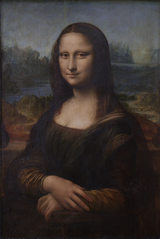
\includegraphics[width=2cm]{figs/monalisa}};
	\node[below=0 of mona, text=olivish] {{\tt monalisa.jpg}};

	% monalisa grid
	\foreach \i in {1,...,10}
	{
		\coordinate (x\i) at ($(mona.north)+(0,-2.7*\i mm)$);
		\draw[very thin, draw=black!10] (mona.west |- x\i) -- (mona.east |- x\i);

		\coordinate (y\i) at ($(mona.west)+(1.85*\i mm,0)$);
		\draw[very thin,draw=black!10] (mona.north -| y\i) -- (mona.south -| y\i);
	}

	% Tail
	\draw[cursor, <-, draw=blackish] (a4) -- +(0, 14mm)
		node[midway, right, text=blackish] (t) {Tail}
		node[TP, at end, above] (producer) {Producer thread};

	\draw[cursor, draw=olivish] (producer) to[out=180, in=0] (mona);

	% tv and monalisa output
	\node[below right=-10mm and 30mm of a4, inner sep = 0] (tv)
		{
\includegraphics[width=4cm]{figs/tv}};
	\node[below right=-5mm and 8mm of tv.west, inner sep = 0] (mona2)
		{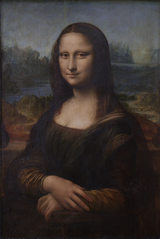
\includegraphics[width=10mm]{figs/monalisa}};

	% Head
	\draw[cursor, ->, draw=blackish]  (a2) -- +(0,-17mm)
		node[midway, right, text=blackish] (h) {Head}
		node[TC, at end, below] (consumer) {Consumer thread};
	\draw[cursor, draw=magentish, ->] (consumer) to[out=0, in=180] (tv);

	\end{tikzpicture}
	\end{center}
\end{frame}


\frame{
	\structure{\Huge Coding session \#1}\\~\\
	Implementing an SPSC ringbuffer\ldots
}
% Copyright (C) Huawei Technologies Co., Ltd. 2024. All rights reserved.
% SPDX-License-Identifier: MIT
\begin{frame}[fragile]{\Large So, what is the problem, again?}
	\begin{columns}[T]
		\column{.5\textwidth}{%
			\begin{lstlisting}
            #define N 8
            item_t *A[N];
            uint Tail = 0, Head = 0;\end{lstlisting}
			
\begin{tikzpicture}[%
					remember picture,
					itemsz/.style={minimum width = 5mm, minimum height = 5mm},
					item/.style={very thick, draw, itemsz, outer sep=0},
					cursor/.style={very thick,<-, font=\ttfamily},
				]%
				\useasboundingbox[draw=pltgreen, ultra thick, rounded corners] (-.3\textwidth,-.30\textheight) rectangle (.7\textwidth,.3\textheight);
				\node[item, fill on={<2-5>}{olivish}, fill on={<6->}{magentish}] (a1) {};
				\node[item, fill on={<3-6>}{olivish}, fill on={<7->}{magentish}, right=0 of a1] (a2) {};
				\node[item, fill on={<4-7>}{olivish}, fill on={<8->}{magentish}, right=0 of a2] (a3) {};
				\node[item, fill on={<16>}{olivish}, fill on={<15>}{magentish}, fill on={<17>}{magentish}, right=0 of a3] (a4) {};
				\node[item, right=0 of a4] (a5) {};
				\node[item, right=0 of a5] (a6) {};
				\node[item, right=0 of a6] (a7) {};
				\node[item, right=0 of a7] (a8) {};
				\node[left=1mm of a1] {A =};

				% insert a few items
				\draw<1>[cursor] (a1) -- +(0, 1) node[at end, right] {Tail};
				\draw<2>[cursor] (a2) -- +(0, 1) node[at end, right] {Tail};
				\draw<3>[cursor] (a3) -- +(0, 1) node[at end, right] {Tail};
				\draw<4-10>[cursor] (a4) -- +(0, 1) node[at end, right] (t) {Tail};

				% consume a few items
				\draw<-5>[cursor] (a1) -- +(0,-1) node[at end, right] {Head};
				\draw<6>[cursor]  (a2) -- +(0,-1) node[at end, right] {Head};
				\draw<7>[cursor]  (a3) -- +(0,-1) node[at end, right] {Head};
				\draw<8-13>[cursor] (a4) -- +(0,-1) node[at end, right] (h) {Head};

				% alice and bob
				\node<11-16>[above=0mm of a4, text=olive] {t};
				\draw<11->[cursor] (a5) -- +(0, 1) node[at end, right] (t) {Tail};
				\draw<14->[cursor] (a5) -- +(0,-1) node[at end, right] (h) {Head};
				\node<14>[below=0mm of a4, text=magenta] {h};

				\node<9->[alicetxt, above=0 of t] (alice) {Producer};
				\node<9->[bobtxt, below=0 of h] (bob) {Consumer};

			\end{tikzpicture}%
		}\column{.5\textwidth}{%
			\vspace{2mm}
			\begin{lstlisting}
bool enqueue(item_t *item) {
    // space to enqueue?
    @\coord{e1}@if (Tail - Head == N)
        return false;
    @\coord{e2}@uint t = Tail@\only<-16>{++}@;
    @\coord{e3}@A[t % N] = item;
@\only<17>{~~~~\hspace{1ex}\coord{ex}@Tail = t + 1;@\newline}@    @\coord{e4}@return true;
}\end{lstlisting}\pause\pause\pause\pause
			\begin{lstlisting}
item_t *dequeue() {
    // item to dequeue?
    @\coord{d1}@if (Tail - Head == 0)
        return NULL;
    @\coord{d2}@uint h = Head@\only<-16>{++}@;
    @\coord{d3}@item_t *i = A[h % N];
@\only<17>{~~~~\hspace{1ex}\coord{dx}@Head = h + 1;@\newline}@    @\coord{d4}@return i;
}
        \end{lstlisting}

        \only<17>{\vspace{-4mm}}

		}%
	\end{columns}
	\begin{tikzpicture}[overlay, remember picture,
			bp/.style={<-, ultra thick},
			bx/.style={<-, dashed, thin},
		]
		\draw<9>[bp,olive] (e1) -- +(-5mm,0);
		\draw<10>[bp,olive] (e2) -- +(-5mm,0);
		\draw<11>[bp,olive] (e3) -- +(-5mm,0);
		\draw<12-15>[bx,olive] (e3) -- +(-5mm,0);
		\draw<16>[bp,olive] (e4) -- +(-5mm,0);
		\draw<12>[bp,magenta] (d1) -- +(-5mm,0);
		\draw<13>[bp,magenta] (d2) -- +(-5mm,0);
		\draw<14>[bp,magenta] (d3) -- +(-5mm,0);
		\draw<15>[bp,magenta] (d4) -- +(-5mm,0);
		\draw<16>[bx,magenta] (d4) -- +(-5mm,0);
		\node<15-16>[left=5mm of bob, warning] {Read garbage!};
		\draw<17>[pltgreen, ultra thick] (d2) -- +(-5mm, 0);
		\draw<17>[pltgreen, ultra thick] (dx) -- +(-5mm, 0);
		\draw<17>[pltgreen, ultra thick] (e2) -- +(-5mm, 0);
		\draw<17>[pltgreen, ultra thick] (ex) -- +(-5mm, 0);

	\end{tikzpicture}
\end{frame}

\frame{
	\structure{\Huge Coding session \#2}\\~\\

	Would this work on Raspberry Pi?\\
}

\section{Weak Memory Models}
% Copyright (C) Huawei Technologies Co., Ltd. 2024. All rights reserved.
% SPDX-License-Identifier: MIT
\begin{frame}[fragile]{Weak Memory Consistency Models (WMMs)}
	\begin{columns}[c]
		\column{.5\textwidth}{%
			\centering
			\begin{itemize}\setlength{\itemindent}{-1em}
				\item Modern architectures becoming popular\\ \eg, {Arm}, {RISC-V}\\[8pt]
				\item<7-> {\bf Aggressive reorderings} to improve sequential performance\\[8pt]
					%\item<7-> Nightmare for concurrent code!
				\item<7-> {\bf Much higher non-determinisim};\\
					even harder to test!\\[8pt]
				\item<7-> Careful use of {\bf memory barriers}\\ (neither too many, nor too few)
			\end{itemize}
			%\resizebox{.5\textwidth}{!}{\input{figs/store-buffering}}
			%\uncover<7->{\hspace{-10mm}\resizebox{.9\textwidth}{!}{% Copyright (C) Huawei Technologies Co., Ltd. 2024. All rights reserved.
% SPDX-License-Identifier: MIT
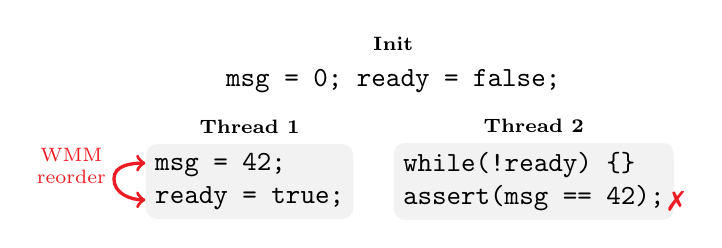
\begin{tikzpicture}[
    a/.style = {->, thick},
    j/.style = {fill=white, font=\scriptsize\bf},
    b/.style = {rounded corners, align=left}, %, text width = 7mm},
    i/.style = {b},
    t/.style = {b, fill=light gray},
    c/.style = {b, fill=light red, text width=34mm},
    ]
\coordinate (x);
\node[i, above=10mm of x] (a) {\verb|msg = 0; ready = false;|};
\node[t, left=5mm of x] (b1) {\verb|msg = 42;|\\ \verb|ready = true;|};
\node[t, right=0mm of x] (b2) {\verb|while(!ready) {}|\\{\verb|assert(msg == 42);|}};
%\node[c, below=of x] (c) {\verb+assert(a != 0 || b != 0);+};
%\draw[a]  (a) -- (b1);
%\draw[a]  (a) -- (b2);
%\draw[a]  (b1) -- (c);
%\draw[a]  (b2) -- (c);
%\node[j, below=1mm of a] {{\tt pthread_create}};
%\node[j, above=1mm of c] {{\tt pthread_join}};
\node[j, above=0 of a] {Init};
\node[j, fill=none, above=0 of b1] (t1) {Thread 1};
\node[j, fill=none, above=0 of b2] (t2) {Thread 2};
\node[text=HuaweiRed, right=-2mm of b2.south east, yshift=2.5mm] {\xmark};

%\draw[a]  (a) -- (t1);
%\draw[a]  (a) -- (t2);
\draw<1->[<->, very thick, HuaweiRed] (b1.170) to [out=180, in = 90]
node[midway, left=1mm, align=center, font=\scriptsize] {WMM\\reorder}
+(-4mm, -2mm) to [out = -90, in = 180] (b1.190);
\end{tikzpicture}
}}
		}\column{.5\textwidth}{%
			\centering
			%\only<-7>{\resizebox{!}{.8\textheight}{%
			\only<-7>{\resizebox{.8\textwidth}{!}{%
					\begin{tikzpicture}[cut/.style={draw, very thick,fill=white}]
						\draw[draw=none, dotted, use as bounding box] (0cm,-48mm) rectangle (8cm, 48mm);
						\node<2-7>[cut] at (35mm, 25mm) (a1) {
\includegraphics[width=7cm]{figs/arm-huawei}};
						\node<3-7>[cut, below right=13mm and -1cm of a1.north] (a2) {
\includegraphics[width=7cm]{figs/arm-amazon}};
						\node<4-7>[cut, below left=18mm and -2mm of a2.north] (a3) {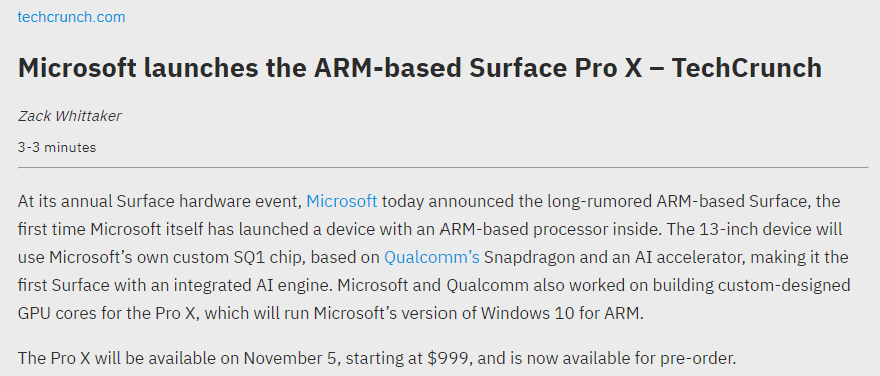
\includegraphics[width=7cm]{figs/arm-microsoft}};
						\node<5-7>[cut, below right=15mm and -28mm of a2.north] (a3) {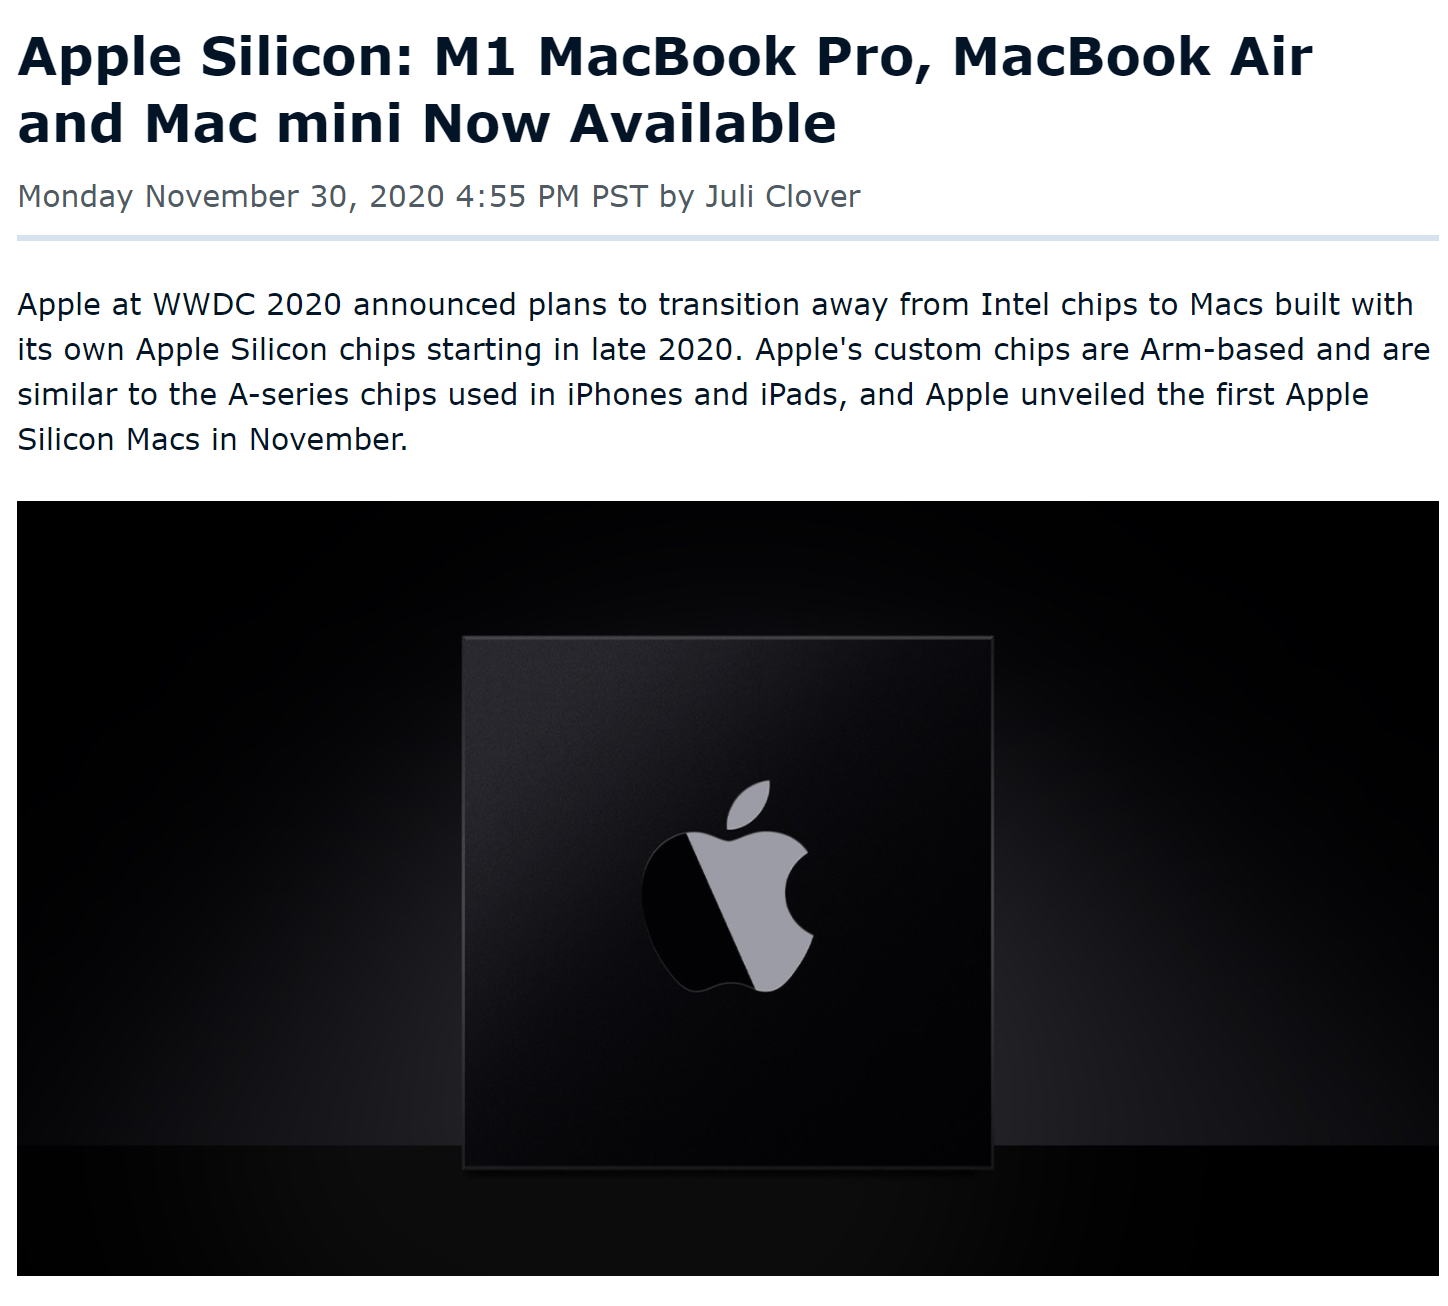
\includegraphics[width=7cm]{figs/arm-apple}};
						\node<6-7>[cut, below right=35mm and -8cm of a2.north] (a4) {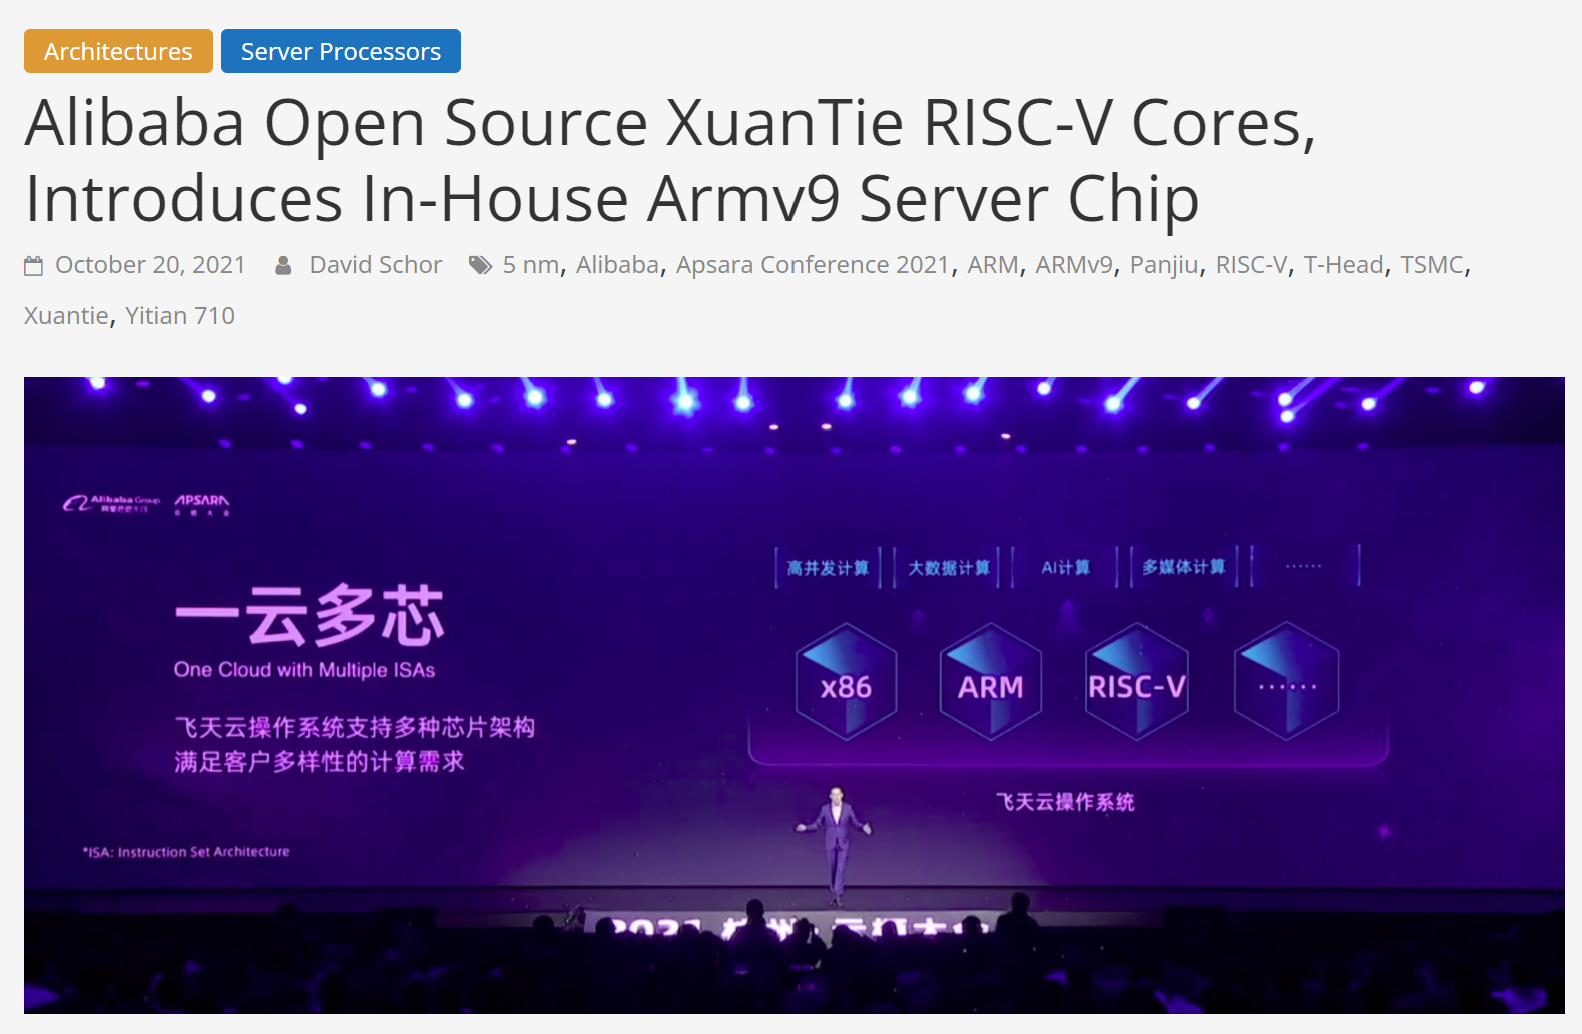
\includegraphics[width=7cm]{figs/arm-alibaba.png}};
					\end{tikzpicture}}}%
		}
	\end{columns}
\end{frame}

% Copyright (C) Huawei Technologies Co., Ltd. 2024. All rights reserved.
% SPDX-License-Identifier: MIT
\begin{frame}[fragile]{How did WMM behavior break {\tt ccat}?}

\begin{columns}
\column{.5\textwidth}{%
	\begin{itemize}\large
		\item Independent memory accesses\\
			can be reordered\\[8pt]
		\item For example, reorders writes\\
			to \lstinline|A[t % N]| and \lstinline|Tail|\\[8pt]
		\item<2-> We need to add barriers\\[8pt]
		\item<5> {\bf Not so simple}:
			\begin{itemize}
			\item How many barriers?
			\item Where exactly?
			\item Dependencies
			\end{itemize}
	\end{itemize}
}\column{.5\textwidth}{%
	\begin{lstlisting}
bool enqueue(item_t *item) {
    // space to enqueue?
   @\coord{We1}@if (Tail - Head == N)
       return false;
   @\coord{We2}@uint t = Tail;
   @\coord{We3}@A[t % N] = item;
   @\coord{Wex}@Tail =|@\only<2->{@rel@}@| t + 1;
   @\coord{We5}@return true;
}

item_t *dequeue() {
    // item to dequeue?
   @\coord{Wd1}@if (Tail|@\only<2->{@acq@}@| - Head == 0)
       return NULL;
   @\coord{Wd2}@uint h = Head;
   @\coord{Wd3}@item_t *i = A[h % N];
   @\coord{Wdx}@Head =|@\only<2->{@rel@}@| h + 1;
   @\coord{Wd4}@return i;
}
\end{lstlisting}
}%
\end{columns}

\begin{tikzpicture}[overlay, remember picture,
		bp/.style={<-, ultra thick},
		bx/.style={<-, dashed, thin},
	]
	\draw[draw=none] (We3) -- (Wex) node[midway] (pe) {};
	\draw[draw=none] (Wd3) -- (Wdx) node[midway] (pd) {};
	\draw<1>[<->, very thick] (We3.170)
		-- ($(pe)+(-5mm,0)$)
		-- (Wex.190);

	\draw<3-4>[draw=blue, very thick, ->] (Wex) --
		node[midway, above=0, font=\tiny] {release}
		+(-1,0) to[out=180, in=180] (\tikztostart|-Wd1) --
		node[midway, below=0, font=\tiny] {acquire}
		(Wd1) ;
	\node<3-4>[between=Wex and Wd1, xshift=-15mm, align=center,fill=white, font=\tiny]  {preserved\\ program order};



	\draw<3>[draw=pltred, very thick, <-]
			($(We3)+(22mm,0)$)
			to[out=-10, in=100]
			+(1,-8mm)
			to[out=-80, in=40]
			node[font=\tiny, at start, right,align=center] {write after\\read (fre)}
			($(Wd3)+(26mm,0)$);

	\draw<4>[draw=pltgreen, very thick, ->]
			($(We3)+(22mm,0)$)
			to[out=-10, in=100]
			+(1,-8mm)
			to[out=-80, in=40]
			node[font=\tiny, at start, right,align=center] {reads\\from}
			($(Wd3)+(26mm,0)$);

\end{tikzpicture}
\end{frame}

\frame{
	\structure{\Huge Coding session \#3}\\~\\

	How to relax barriers without breaking the code?\\
}
\frame{%
	\begin{block}{{\Large Agenda}}%
	\begin{itemize}\Large
		\item {\hide Introduction}
		\item {\hide Part 1: Concurrent Monalisa}
		\item {\unhide Part 2: {\tt vsyncer} to the rescue}
		\item {\hide Outlook}
	\end{itemize}
	\end{block}
}
% Copyright (C) Huawei Technologies Co., Ltd. 2024. All rights reserved.
% SPDX-License-Identifier: MIT

\begin{frame}<\theframerange>[fragile]{Safe and Fast Concurrency on Arm processors}
    \framesubtitle{%
    {VSync: Push-button Verification and Optimization on WMMs --- \award Distinguished paper at ASPLOS'21}}

    \vspace{1mm}

\begin{tikzpicture}[
        base/.style={anchor=center, align=center},
        %cmpt/.style={base, fill=blue!60!black!20, rounded corners, text=black, minimum width=15mm, minimum height=10mm},
        cmpt/.style={base, fill=libvsync!30, rounded corners, text=black, minimum width=15mm, minimum height=10mm},
        novel/.style={cmpt, fill=vsyncer!40},
        cmd/.style={base, fill=gray!20, text=black, font=\ttfamily},
        file/.style={base, dashed, thin, fill=blue!20!black!20},
        ar/.style={thick, align=center, font=\scriptsize},
        bx/.style={minimum width=7mm, minimum height=5mm},
        safer/.style={->, thick, draw=red!70!black, text=red!70!black },
        faster/.style={<-, thick, draw=blue!70!black, text=blue!70!black },
    ]

    \draw[use as bounding box, draw=none, dotted] (-15mm, -.3\textheight) rectangle (12cm, .1\textheight);
    %\node<-10>[file,align=center] (impl) {target.c};
    \node[file,align=center] (impl) {target.c};
    \node[below=19mm of impl.center, cmpt] (atomics) {\libvsync\\atomics};
    \node[right=25mm of impl.center, cmd, rounded corners] (clang) {clang\\$\ge v14.0$};
    \node[below right=19mm and 25mm of clang.center, novel] (analyzer) {barrier\\analyzer};
    \node[above right=19mm and 25mm of analyzer.center, novel] (mutator) {mutation\\checker};
    %\node<-10>[right=35mm of mutator.center, novel] (genmc) {model\\checker};
    \node[right=35mm of mutator.center, novel] (genmc) {model\\checker};

    %\node<-10>[below=19mm of clang.center, file, align=center] (gen) {test\_case.c};
    \node[below=19mm of clang.center, file, align=center] (gen) {test\_case.c};
    \node[right=30mm of analyzer.center, novel] (optimizer) {barrier\\optimizer};%
    \node[right=30mm of optimizer.center, file] (output) {optimization\\report};

    \draw[->, ar] (impl) -- (clang);
    \draw[->, ar] (gen) --
    (clang);
    \draw[->, ar] (clang) -- node[midway, above] {input IR} (mutator);
    \draw[->, ar] (clang -| analyzer) -- (analyzer);

    \draw[->, ar] (mutator.9) --
    node[midway, above] {mutated IR}
    (genmc.170);
    \draw[<-, ar] (mutator.-9) --
    node[midway, below] {result}
    (genmc.-170);

    \draw[->, ar] (analyzer) --
    node[midway, below] { \#barriers}
    (optimizer);

    \draw[->, ar] (optimizer.135) --
    node[midway, left=1mm, align=center] {barrier-mode\\combination}
    (mutator.-135);
    \draw[<-, ar] (optimizer.45) --
    node[midway, right=1mm] {status}
    (mutator.-45);

    \draw[->, ar] (optimizer) -- (output);
    \draw[->, ar] (atomics) -- (impl);

    \coordinate[below left=7mm and 12mm of atomics.center] (l1);
    \coordinate[above left=9mm and 12mm of atomics.center] (l11);
    \coordinate[above left=26mm and 9mm of analyzer.center] (l12);
    \coordinate[below left=7mm and 9mm of analyzer.center] (l2);
    \coordinate[above right=7mm and 10mm of genmc.center] (r1);
    \coordinate[below right=7mm and 10mm of genmc.center] (r2);
    \coordinate[below left=7mm and 10mm of genmc.center] (r3);
    \coordinate[below right=7mm and 12mm of optimizer.center] (r4);
    \draw[dashed, draw=vsyncer] (l12) -- (r1) -- (r2) -- (r3) -- (r4) -- (l2) -- cycle;
    \node[above=2mm of mutator] {\vsyncer};

    \node<2>[fill=gray!10, rounded corners, draw=black, ultra thick, left=-10mm of mutator, align=center] (e) {
        \begin{adjustbox}{width=5cm,keepaspectratio}
        % Copyright (C) Huawei Technologies Co., Ltd. 2024. All rights reserved.
% SPDX-License-Identifier: MIT
\begin{lstlisting}[language=C, style=compact,escapeinside={//*}{\^^M}]
// TTAS lock implementation
// using VSync atomics (SC)

typedef atomic_t lock_t;
void lock_acquire(lock_t *lock) {
    do {
        while(vatomic_read(lock));//* \label{ln:ttas-await}
    } while(vatomic_xchg(lock, 1));//* \label{ln:ttas-xchg}
}
void lock_release(lock_t *lock) {
    vatomic_write(lock, 0); //* \label{ln:ttas-write}
}
\end{lstlisting}

 \end{adjustbox}
    };
    \draw<2>[->, ultra thick, gray] (impl) to [bend left] (e);
    \node<3-9>[fill=gray!10, rounded corners, draw=white, ultra thick, above=0 of impl, align=center] (e) {
        \begin{adjustbox}{width=2cm,keepaspectratio}
        % Copyright (C) Huawei Technologies Co., Ltd. 2024. All rights reserved.
% SPDX-License-Identifier: MIT
\begin{lstlisting}[language=C, style=compact,escapeinside={//*}{\^^M}]
// TTAS lock implementation
// using VSync atomics (SC)

typedef atomic_t lock_t;
void lock_acquire(lock_t *lock) {
    do {
        while(vatomic_read(lock));//* \label{ln:ttas-await}
    } while(vatomic_xchg(lock, 1));//* \label{ln:ttas-xchg}
}
void lock_release(lock_t *lock) {
    vatomic_write(lock, 0); //* \label{ln:ttas-write}
}
\end{lstlisting}

 \end{adjustbox}
    };


    %% barrier mappings
    \node<4>[fill=gray!10, rounded corners, draw=black, ultra thick, align=center, font=\tiny] at (75mm,5mm)  (nox) {
        \begin{adjustbox}{width=10cm,keepaspectratio}
        % Copyright (C) Huawei Technologies Co., Ltd. 2024. All rights reserved.
% SPDX-License-Identifier: MIT
\begin{tabular}{l|lll}
    \small {\tt\color{libvsync} vatomic} & \small RISC-V & \small ARMv8 & \small x86
    \\
    \hline\\[-6pt]
    \lstinline[language=C,style=compact]|vatomic_xchg| & \lstinline[language={C},style=compact]|amoswap.w.aq.rl.sc| & %\lstinline[style=compact]|SWPAL| or
    \lstinline[style=compact]|LDAXR;STLXR| & \lstinline[style=compact]|XCHG |\\
    \lstinline[language=C,style=compact]|vatomic_xchg_rel| & \lstinline[language={C},style=compact]|amoswap.w.rl| & %\lstinline[style=compact]|SWPL| or
    \lstinline[style=compact]|LDXR;STLXR| & \lstinline[style=compact]|XCHG |\\
    \lstinline[language=C,style=compact]|vatomic_xchg_acq| & \lstinline[language={C},style=compact]|amoswap.w.aq| & %\lstinline[style=compact]|SWPA| or
    \lstinline[style=compact]|LDAXR;STXR| & \lstinline[style=compact]|XCHG |\\
    \lstinline[language=C,style=compact]|vatomic_xchg_rlx| & \lstinline[language={C},style=compact]|amoswap.w| & %\lstinline[style=compact]|SWP| or
    \lstinline[style=compact]|LDXR;STXR|  & \lstinline[style=compact]|XCHG|\\
    \lstinline[language=C,style=compact]|vatomic_read| & \lstinline[language={C},style=compact]|fence [rw,rw];  lw; fence [r,rw]| & \lstinline[style=compact]|LDAR| & \lstinline[style=compact]|MOV |\\
    \lstinline[language=C,style=compact]|vatomic_read_acq| & \lstinline[language={C},style=compact]|lw; fence [r,rw]| & \lstinline[style=compact]|LDAR|  & \lstinline[style=compact]|MOV|\\
    \lstinline[language=C,style=compact]|vatomic_read_rlx| & \lstinline[language={C},style=compact]|lw| &  \lstinline[style=compact]|LDR|  & \lstinline[style=compact]|MOV|\\
    \lstinline[language=C,style=compact]|vatomic_write| & \lstinline[language={C},style=compact]|fence [rw,w]; sw; fence [rw,rw]| & \lstinline[style=compact]|STLR|  & \lstinline[style=compact]|MOV;MFENCE|\\
    \lstinline[language=C,style=compact]|vatomic_write_rel| & \lstinline[language={C},style=compact]|fence [rw,w]; sw| & \lstinline[style=compact]|STLR|  & \lstinline[style=compact]|MOV|\\
    \lstinline[language=C,style=compact]|vatomic_write_rlx| & \lstinline[language={C},style=compact]|sw| & \lstinline[style=compact]|STR| & \lstinline[style=compact]|MOV|\\
    \hline\\[-6pt]
    \lstinline[language=C,style=compact]|vatomic_fence| & \lstinline[language={C},style=compact]|fence [rw,rw]| & \lstinline[style=compact]|DMB ISH|  & \lstinline[style=compact]|MFENCE|\\
    \lstinline[language=C,style=compact]|vatomic_fence_acq| & \lstinline[language={C},style=compact]|fence [r,rw]| & \lstinline[style=compact]|DMB ISHLD| & \lstinline[style=compact]|NOP |\\
    \lstinline[language=C,style=compact]|vatomic_fence_rel| & \lstinline[language={C},style=compact]|fence [rw,w]| & \lstinline[style=compact]|DMB ISH| & \lstinline[style=compact]|NOP |\\
    \lstinline[language=C,style=compact]|vatomic_fence_rlx| & \lstinline[language={C},style=compact]|nop| & \lstinline[style=compact]|NOP| & \lstinline[style=compact]|NOP|
\end{tabular}
 \end{adjustbox}
    };
    \draw<4>[->, ultra thick, gray] (atomics) to [bend left] (nox.west);
    \node<5-9>[fill=gray!10, rounded corners, draw=white, ultra thick, below=0 of atomics, align=center] (e) {
        \begin{adjustbox}{width=2cm,keepaspectratio}
        % Copyright (C) Huawei Technologies Co., Ltd. 2024. All rights reserved.
% SPDX-License-Identifier: MIT
\begin{tabular}{l|lll}
    \small {\tt\color{libvsync} vatomic} & \small RISC-V & \small ARMv8 & \small x86
    \\
    \hline\\[-6pt]
    \lstinline[language=C,style=compact]|vatomic_xchg| & \lstinline[language={C},style=compact]|amoswap.w.aq.rl.sc| & %\lstinline[style=compact]|SWPAL| or
    \lstinline[style=compact]|LDAXR;STLXR| & \lstinline[style=compact]|XCHG |\\
    \lstinline[language=C,style=compact]|vatomic_xchg_rel| & \lstinline[language={C},style=compact]|amoswap.w.rl| & %\lstinline[style=compact]|SWPL| or
    \lstinline[style=compact]|LDXR;STLXR| & \lstinline[style=compact]|XCHG |\\
    \lstinline[language=C,style=compact]|vatomic_xchg_acq| & \lstinline[language={C},style=compact]|amoswap.w.aq| & %\lstinline[style=compact]|SWPA| or
    \lstinline[style=compact]|LDAXR;STXR| & \lstinline[style=compact]|XCHG |\\
    \lstinline[language=C,style=compact]|vatomic_xchg_rlx| & \lstinline[language={C},style=compact]|amoswap.w| & %\lstinline[style=compact]|SWP| or
    \lstinline[style=compact]|LDXR;STXR|  & \lstinline[style=compact]|XCHG|\\
    \lstinline[language=C,style=compact]|vatomic_read| & \lstinline[language={C},style=compact]|fence [rw,rw];  lw; fence [r,rw]| & \lstinline[style=compact]|LDAR| & \lstinline[style=compact]|MOV |\\
    \lstinline[language=C,style=compact]|vatomic_read_acq| & \lstinline[language={C},style=compact]|lw; fence [r,rw]| & \lstinline[style=compact]|LDAR|  & \lstinline[style=compact]|MOV|\\
    \lstinline[language=C,style=compact]|vatomic_read_rlx| & \lstinline[language={C},style=compact]|lw| &  \lstinline[style=compact]|LDR|  & \lstinline[style=compact]|MOV|\\
    \lstinline[language=C,style=compact]|vatomic_write| & \lstinline[language={C},style=compact]|fence [rw,w]; sw; fence [rw,rw]| & \lstinline[style=compact]|STLR|  & \lstinline[style=compact]|MOV;MFENCE|\\
    \lstinline[language=C,style=compact]|vatomic_write_rel| & \lstinline[language={C},style=compact]|fence [rw,w]; sw| & \lstinline[style=compact]|STLR|  & \lstinline[style=compact]|MOV|\\
    \lstinline[language=C,style=compact]|vatomic_write_rlx| & \lstinline[language={C},style=compact]|sw| & \lstinline[style=compact]|STR| & \lstinline[style=compact]|MOV|\\
    \hline\\[-6pt]
    \lstinline[language=C,style=compact]|vatomic_fence| & \lstinline[language={C},style=compact]|fence [rw,rw]| & \lstinline[style=compact]|DMB ISH|  & \lstinline[style=compact]|MFENCE|\\
    \lstinline[language=C,style=compact]|vatomic_fence_acq| & \lstinline[language={C},style=compact]|fence [r,rw]| & \lstinline[style=compact]|DMB ISHLD| & \lstinline[style=compact]|NOP |\\
    \lstinline[language=C,style=compact]|vatomic_fence_rel| & \lstinline[language={C},style=compact]|fence [rw,w]| & \lstinline[style=compact]|DMB ISH| & \lstinline[style=compact]|NOP |\\
    \lstinline[language=C,style=compact]|vatomic_fence_rlx| & \lstinline[language={C},style=compact]|nop| & \lstinline[style=compact]|NOP| & \lstinline[style=compact]|NOP|
\end{tabular}
 \end{adjustbox}
    };

    \node<6>[fill=gray!10, rounded corners, draw=black, ultra thick, right=-20mm of mutator, align=center] (e) {
        \begin{adjustbox}{width=5cm,keepaspectratio}
        % Copyright (C) Huawei Technologies Co., Ltd. 2024. All rights reserved.
% SPDX-License-Identifier: MIT
\begin{lstlisting}[language=C, style=compact]
lock_t lock;
int v = 0; // shared state
void run(int id) {
    lock_acquire(&lock);
    v++; // critical sec.
    lock_release(&lock);
}

void main() {
    pthread_t t[N]; // N == 3
    for (int i=0; i < N; i++)
        pthread_create(&t[i], 0, run, i);
    for (int i=0; i < N; i++)
        pthread_join(t[i], 0);
    assert (v == N); // check of ME
}
\end{lstlisting}

%\begin{lstlisting}[language=C, style=compact]
%lock_t lock;
%int v = 0; // shared state
%void run(int id) {
%    do {
%        lock_acquire(&lock);
%        v++; // critical sec.
%        lock_release(&lock);
%    } while (id++ == 0);
%}
%
%void main() {
%    pthread_t t[N]; // N == 3
%    for (int i=0; i < N; i++)
%        pthread_create(&t[i], 0, run, i);
%    for (int i=0; i < N; i++)
%        pthread_join(t[i], 0);
%    assert (v == N+1); // check of ME
%}
%\end{lstlisting}
 \end{adjustbox}
    };
    \draw<6>[->, ultra thick, gray] (gen) to [bend left] (e);
    \node<7-9>[fill=gray!10, rounded corners, draw=white, ultra thick, below=0 of gen, align=center] (e) {
        \begin{adjustbox}{width=2cm,keepaspectratio}
        % Copyright (C) Huawei Technologies Co., Ltd. 2024. All rights reserved.
% SPDX-License-Identifier: MIT
\begin{lstlisting}[language=C, style=compact]
lock_t lock;
int v = 0; // shared state
void run(int id) {
    lock_acquire(&lock);
    v++; // critical sec.
    lock_release(&lock);
}

void main() {
    pthread_t t[N]; // N == 3
    for (int i=0; i < N; i++)
        pthread_create(&t[i], 0, run, i);
    for (int i=0; i < N; i++)
        pthread_join(t[i], 0);
    assert (v == N); // check of ME
}
\end{lstlisting}

%\begin{lstlisting}[language=C, style=compact]
%lock_t lock;
%int v = 0; // shared state
%void run(int id) {
%    do {
%        lock_acquire(&lock);
%        v++; // critical sec.
%        lock_release(&lock);
%    } while (id++ == 0);
%}
%
%void main() {
%    pthread_t t[N]; // N == 3
%    for (int i=0; i < N; i++)
%        pthread_create(&t[i], 0, run, i);
%    for (int i=0; i < N; i++)
%        pthread_join(t[i], 0);
%    assert (v == N+1); // check of ME
%}
%\end{lstlisting}
 \end{adjustbox}
    };

    \node<8>[fill=gray!10, rounded corners, draw=black, ultra thick, left=0 of mutator, align=center] (e) {
        \begin{adjustbox}{width=4cm,keepaspectratio}
        % Copyright (C) Huawei Technologies Co., Ltd. 2024. All rights reserved.
% SPDX-License-Identifier: MIT
\begin{lstlisting}[style=compact]
optimization report
-------------------

lock_acquire
  vatomic_read --> rlx
  vatomic_xchg --> acq

lock_release
  vatomic_write --> rel
\end{lstlisting}


 \end{adjustbox}
    };
    \draw<8>[->, ultra thick, gray] (output) to [bend right] (e);
    \node<9>[fill=gray!10, rounded corners, draw=white, ultra thick, below=0 of output, align=center] (e) {
        \begin{adjustbox}{width=2cm,keepaspectratio}
        % Copyright (C) Huawei Technologies Co., Ltd. 2024. All rights reserved.
% SPDX-License-Identifier: MIT
\begin{lstlisting}[style=compact]
optimization report
-------------------

lock_acquire
  vatomic_read --> rlx
  vatomic_xchg --> acq

lock_release
  vatomic_write --> rel
\end{lstlisting}


 \end{adjustbox}
    };

    %\node<9>[above=7mm of mutator, text width=7cm, rounded corners,
    %draw=red, align=center, very thick] {%
    %{\bf Problem}: Some optimizations cause hangs on Arm CPUS! Why?};
    %\draw<10->[red, very thick] (optimizer) to[out=-90, in=90] +(-1,-15mm) node[below, rounded corners, fill=red, text=white, font=\bf, align=center] {Adaptive Linear Relaxation};
%    \draw<9> [fill=black!30, opacity=0.6, draw=none, rounded corners]
%    (-1.8,1.5) -- (12,1.5) -- (12,-2.8) -- (8.7, -2.8) -- (8.7, -1) -- (6.3, -1) -- (6.3, -2.8) -- (-1.8, -2.8) -- cycle;

    \node<10>[
        line width=1mm, rounded corners, draw=red!90!black,
        fill=white, text=black,
        text width=100mm, align=left,
        font=\footnotesize,
        below left=10mm and 120mm of genmc.center,
        anchor=west
    ] (best)
    {%
        \vspace{2mm}

        {\large Under the hood the {\bf best model checkers} for WMMs}\\

        \begin{block}{\bf \footnotesize GenMC by MPI-SWS}
            \begin{itemize}\setlength\itemindent{-1em}\footnotesize
                \item \url{https://github.com/MPI-SWS/genmc}
                \item First to verify liveness of spinloops based on our work.
            \end{itemize}
        \end{block}
        \begin{block}{\bf \footnotesize Dartagnan by TU Braunschweig and Huawei DRC}
            \begin{itemize}\setlength\itemindent{-1em}\footnotesize
                \item \url{https://github.com/hernanponcedeleon/Dat3M}
                \item Hernan Ponce de Leon (maintainer) joined our team in 2022
                \item We are transforming it from an academic into a practical tool
                \item \hspace{-2mm}\award\hspace{2mm} Gold medal at SV-COMP 2023
                \item \hspace{-2mm}\award\hspace{-2mm}\award\hspace{2mm} Two gold medals at SV-COMP 2024
            \end{itemize}
        \end{block}
    };
    \draw<10>[<-, red, line width=1mm] (genmc) to[out=90, in = 0] (best.25);

\end{tikzpicture}
\end{frame}



\frame{
	\structure{\Huge Coding session \#4}\\~\\

	What if MPMC? ARMv8? \ldots
}

\section{Outlook}
\frame{%
	\begin{block}{{\Large \bf Agenda}}%
	\begin{itemize}\Large
		\item {\hide Introduction}
		\item {\hide Part 1: Concurrent Monalisa}
		\item {\hide Part 2: {\tt vsyncer} to the rescue}
		\item {\unhide Outlook}
	\end{itemize}
	\end{block}
}

{\nofootline\frame{
	\structure{\Huge Do we have to always do all that work??}
}}

% Copyright (C) Huawei Technologies Co., Ltd. 2024. All rights reserved.
% SPDX-License-Identifier: MIT
\begin{frame}<\theframerange>[fragile]{\libvsync: Solid concurrency foundations}
	\framesubtitle{\url{github.com/open-s4c/libvsync}}

    \begin{columns}[T]
        \column{.7\textwidth}{%
        \resizebox{\textwidth}{!}{%
        \begin{tikzpicture}[
            cmpt/.style = {
            very thick,
            draw,
            minimum width = 20mm,
            minimum height = 11mm,
            rounded corners,
            align = center
            },
            lvsync/.style = {
            cmpt,
            draw=none,
            fill=libvsync!50,
            }]
            \draw[draw=none, dotted, use as bounding box] (-.8\textwidth,-8) rectangle (.8\textwidth,12mm);

            \coordinate (app);
            \node[cmpt,minimum width=45mm, left=1mm of app, anchor=south east]
            (app1) {{\bf Application}};

            \node[cmpt,minimum width=45mm, left=-1mm of app, anchor=south west]
            (db1) {{\bf Database}\\{\small OpenGauss DB}};

            \node[cmpt,below=2mm of app, minimum width=70mm]
            (hm) {{\bf Operating System}\\{\small HongMeng, OpenHarmony, OpenEuler}};

            \node[cmpt,minimum width=92mm, below=60mm of hm]
            (hw) {{\bf Multicore CPU}\\ \arm, \riscv};

            \node<2->[lvsync, minimum width=92mm, above=10mm of hw]
            (a)  {{\bf Atomic Interface}\\ {\tt vatomic\_\{xchg, get\_add\}}};

            \node<4->[lvsync, text width = 25mm, below=29mm of hm, xshift=14mm, , anchor=south east]
            (cds) {{\bf Lockless Data Structures}\\ list, queue, hashtable, etc};

            \node<4->[lvsync, text width=28mm, left=32mm of cds, yshift=-10.3mm, anchor=south west]
            (sync) {{\bf Synchronization Primitives}\\ spinlock, mutex, rwlock, etc};

            \node<4->[lvsync, text width=28mm, right=1mm of cds, yshift=-10.3mm, anchor=south west]
            (smr) {{\bf Safe Memory Reclamation}\\ hazard-pointer, ebr, etc};

            \draw[draw=gray, dashed, very thick] ($(hw)+(-4.5,10mm)$) --
            node[text=gray, midway, fill=white] (hmm) {hardware memory model}
            ($(hw)+(4.5,10mm)$);

            \draw<2>[draw=gray, dashed, very thick] ($(a)+(-4.5,10mm)$) --
            node[text=gray, midway,fill=white] (smm) {software memory model}
            ($(a)+(4.5,10mm)$);

            \draw<3->[draw=gray, dashed, very thick] ($(a)+(-4.5,10mm)$) --
            node[text=gray, midway,fill=white] (smm) {VSync memory model (VMM)}
            ($(a)+(4.5,10mm)$);

            \draw<4->[draw=gray, dashed, very thick] ($(hm)+(-4.5,-10mm)$) --
            node[text=gray, midway,fill=white] (contract) {library contract}
            ($(hm)+(4.5,-10mm)$);

            \draw<1->[->, thick, dashed] (db1) to [out=0, in=180]
            node[at end, right=-10mm] {%
            
\includegraphics[width=35mm]{figs/opengauss.png}
            }
            +(70mm, 0mm);

            \draw<4->[decorate, decoration={brace,amplitude=3mm,mirror}, very thick, color=libvsync] (sync.west|-contract) -- (sync.west|-hmm)
            node[midway, left=2mm] {\battery{6mm}}
            ;

            \draw<1->[->, thick, dashed] (hm.east) to [out=0, in =180]
            node[at end, right] {
\includegraphics[width=4cm]{figs/openeuler-logo.png}}
            +(25mm, -5mm);
            \draw<1->[->, thick, dashed] (hm.-3) to [out=-20, in=180]
            node[at end, right] {
\includegraphics[width=45mm, clip, trim=50 50 50 50]{figs/OpenHarmonyLogo}}
            +(70mm, -15mm);
            \draw<1->[->, thick, dashed] (hm.south east) to [out=-45, in=180]
            node[at end, right] {
\includegraphics[width=10mm]{figs/hm}}
            +(50mm, -25mm);


            \draw<1->[->, thick, dashed] (hw) to[out=0, in=180]
            node[at end, right] {
\includegraphics[width=18mm]{figs/kirin}}
            +(65mm, 5mm);

            \draw<1->[->, thick, dashed] (hw.north east) to [out=45, in=180]
            node[at end, right] {
\includegraphics[width=25mm]{figs/kunpeng}}
            +(70mm, 15mm);

        \end{tikzpicture}}
        }\hfill \column{.5\textwidth}{%

        }
    \end{columns}
\end{frame}

% Copyright (C) Huawei Technologies Co., Ltd. 2024. All rights reserved.
% SPDX-License-Identifier: MIT

\begin{frame}<\theframerange>[fragile]{Take Aways}
\setul{3pt}{.6pt}

\begin{tikzpicture}[
		a/.style={ultra thick, HuaweiRed, |->},
		n/.style={text width = .42\textwidth},
		q1/.style={rounded corners, draw, very thick, fill=darkred, text=white},
		q/.style={font=\Large, align=center},
		w1/.style={fill=white, align=center},
		%w/.style={rounded corners, draw=HuaweiRed, fill=white, align=center},
		w/.style={rounded corners, fill=redish, text=white, align=center},
 	]
 	\draw[draw=none, use as bounding box] (-.1\textwidth, -.15\textheight) rectangle (0.9\textwidth, .5\textheight);
	\node (a) {};
	\coordinate[above right=4cm and 55mm of a] (d);

	\node[q,left=25mm of d] (q1) {%
		Are you building a\\ concurrent system?};
        \node<2->[left=0mm of a] (b) {
\includegraphics[width=6mm]{figs/battery.png}};
        \node<2->[n, above right=5mm and -2mm of a, anchor=north west] (t1) {%
	        \begin{block}{\color{libvsync}\Large libvsync}
		{\scriptsize \url{github.com/open-s4c/libvsync}}
		\end{block}};
	\draw<2->[a, draw=libvsync] (q1) to[out=-90, in=90]
		node[w,midway, fill=libvsync]
		{Use {\bf battle-proven, WMM-verified}\\
		synchronization primitives\\ and concurrent data structures}
	(t1.140);

	\node<3->[q,right=15mm of d] (q2) {%
		Are you designing a new \\concurrent algorithm?};

	\node<4->[right=55mm of a] (c) {
\includegraphics[width=18mm]{figs/smart-robot.jpg}};
	\node<4->[n, above right=5mm and 72mm of a, anchor=north west] (t2) {%
		\begin{block}{\color{vsyncer}\Large vsyncer}
		{\scriptsize \url{github.com/open-s4c/vsyncer}}
		\end{block}};




	\draw<4->[a, draw=vsyncer] (q2) to[out=-90, in=90]
		node[w,midway,fill=vsyncer]
		{Use {\bf atomics} with {\bf seq_cst barriers}.\\
		If performance critical, {\bf optimize} barriers\\
		with a supporting tool!}
	(t2.140);


	\node<5->[below right=5mm and -40mm of t1, text=redish] {Contributions and feedback welcome!};
\end{tikzpicture}

\end{frame}


\makethanks
\end{document}
